% Diese Zeile bitte -nicht- aendern.
\documentclass[course=erap]{aspdoc}

% Packages
\usepackage{amssymb}
\usepackage{xcolor}
\usepackage{pgfplots}

%%%%%%%%%%%%%%%%%%%%%%%%%%%%%%%%%
%% TODO: Ersetzen Sie in den folgenden Zeilen die entsprechenden -Texte-
%% mit den richtigen Werten.
\newcommand{\theGroup}{215} % Beispiel: 42
\newcommand{\theNumber}{A500} % Beispiel: A123
\author{David Csida \and Georgios Merezas \and Fabian Degen}
\date{Sommersemester 2022} % Beispiel: Wintersemester 2019/20
%%%%%%%%%%%%%%%%%%%%%%%%%%%%%%%%%

% Diese Zeile bitte -nicht- aendern.
\title{Gruppe \theGroup{} -- Abgabe zu Aufgabe \theNumber}

\begin{document}
\maketitle

\section{Einleitung}
\subsection{Einführung}
Sei es beim Herstellen einer Verbindung mit einem Server oder das Chatten mit Freunden und Bekannten rund um
den Globus, nie genoss die Kryptographie mehr Relevanz als jetzt. Man möchte nicht, dass die Nachrichten,
die man an seine Geliebten versendet, von einer dritten Person mitgelesen werden können. Darum existieren
kryptographische Verfahren zur Verschlüsselung von Informationen. Eines dieser Verschlüsselungsverfahren ist
Salsa20/20, welches es zu implementieren galt.

\subsection{Funktionsweise Salsa20/20}
Salsa20/20 ist eine Stromchiffre basierend auf einem sogenannten Add-Rotate-XOR-Schema (kurz: ARX-Schema), ins Leben gerufen von
David J. Bernstein.
\\Salsa20/20 verwendet eine 4$\times$4 Matrix bestehend aus vorzeichenlosen 32-bit Little-Endian-Ganzzahlen,
welche durch Add, Rotate und XOR Operationen aus bestimmen Startwerten erzeugt wird.
Auf dieser generierten Matrix wird dann mit der zu verschlüsselnden Nachricht Byte für Byte eine XOR-Operation ausgeführt.

\subsubsection{Der Salsa20-Kern:}
Der Salsa20-Kern ist eine Funktion, welche einen 64-Byte Block generiert, auf dem, wie oben beschrieben, mit 
der zu verschlüsselnden Nachricht Byte für Byte eine XOR-Operation ausgeführt wird. Es werden bei jeder Operation 
zwei Werte der Matrix aufaddiert, links-rotiert und auf diesem Ergebnis mit einem Eintrag $a_{ij}$ der Matrix eine XOR-Operation ausgeführt.
Der Matrix eintrag $a_{ij}$ wird dann mit dem Ergebnis dieser XOR-Operation überschrieben.
Der 64-Byte-Block wird in 20 sogenannten Runden aus einem 256-Bit-Key, einer 64-Bit Nonce und einem 64-Bit 
Counter generiert. Die zwanzig Runden bestehen jeweils aus vier Viertelrunden. Die Viertelrunden unterscheiden sich 
durch die Anzahl der Rotationen, die für jede ARX-Operation ausgeführt werden und durch die Matrix-Einträge, auf die 
diese Operationen angewandt werden. Am Ende jeder Runde wird die Matrix transponiert.
Den Startzustand $S$ für den generierten 64-Byte-Block bildet folgende 4$\times$4 Matrix, wobei $K_i$ den $i$-ten Teil
des Schlüssels bezeichnet. ($K_0$ steht also für die ersten 4 Bytes in Little-Endian-Reihenfolge des Schlüssels, dasselbe gilt analog für die
Nonce $N_i$ und den Counter $C_i$).
\[
    \begin{pmatrix}
    0\text{x}61707865 & K_0 & K_1 & K_2\\
    K_3 & 0\text{x}3320646\text{e} & N_0 & N_1\\
    C_0 & C_1 & 0\text{x}79622\text{d}32 & K_4\\
    K_5 & K_6 & K_7 & 0\text{x}6\text{b}206574
    \end{pmatrix}
\]
Die Konstanten auf der Diagonalen sind für jeden Key und jede Nonce dieselben.
Den zum Schluss ausgegebenen 64-Byte-Block erhält man duch das aufaddieren des 
Ergebnisses der 20 Runden auf den Startzustand $S$.

\subsection{Aufgabenstellung}

\subsubsection{Theoretischer Teil:}
Folgende theoretische Fragen waren zu beantworten:
\begin{itemize}
    \item Wie könnte man das im letzten Schritt einer jeden Salsa20-Kern Runde ineffiziente, stattfindende transponieren der Matrix optimieren?
    \item Was bedeuten die Werte an der Diagonalen des Startzustands?
    \item Erklären der Funktionsweise einer Stromchiffre anhand eines Beispiels. Warum kann man dieselbe Funktion zum Ver- und Entschlüsseln verwenden? Wie müssen die Parameter gewählt werden, damit dies funktioniert? Warum ist der Counter keine Eingabe des Verschlüsselungsalgorithmus?
\end{itemize}

\subsubsection{Praktischer Teil:}
Zu implementieren  war folgende Funktionalität:
\begin{itemize}
    \item Ein Rahmenprogramm welches I/O-Operationen unterstützt, mithilfe derer man eine ganze Datei in den Speicher einlesen und als Pointer an eine Unterfunktion übergeben kann. Selbiges soll auch zum Schreiben eines Speicherbereiches mit bekannter Länge in eine Datei möglich sein.
    \item \textcolor{blue}{void} salsa20\_core (\textcolor{blue} {uint32\_t} output[16] \textcolor{blue}{const uint32\_t} input[16]) \\
    Diese Funktion implementiert den oben beschriebenen Salsa20-Kern. input bezeichnet dabei den Startzustand des Kerns, output den finalen 64-Byte-Block. \\
    \item \textcolor{blue} {void} salsa20\_crypt (\textcolor{blue}{size\_t} mlen, \textcolor{blue} {const uint8\_t} msg[mlen], \textcolor{blue}{uint8\_t} cipher [mlen], \textcolor{blue}{uint32\_t} key[8], \textcolor{blue} {uint64\_t} iv) \\
    Diese Funktion verschlüsselt eine Nachricht msg der Länge mlen mit einem gegebenen Schlüssel Key und einer Nonce (iv) und schreibt das Ergebnis in cipher.
\end{itemize}



\section{Lösungsansatz}
\subsection{Theoretischer Teil}
\subsubsection{Transponieren}

Das Transponieren der Matrix ist Teil des Salsa20-Kern Algorithmus, ist aber nicht sonderlich performant.
Um ihn weiter zu optimieren, kann man anstatt zwanzig Runden, die jeweils eine Transposition enthalten, zehn sogenannte Doppelrunden
ausführen, die jeweils aus einer sogenannten Spaltenrunde und einer Reihenrunde bestehen. Eine Spaltenrunde ist identisch zu einer
Runde wie oben definiert, während eine Reihenrunde die Indizes bei Matrixzugriffen so wählt, dass die Matrix behandelt wird
als wäre sie transponiert.

\subsubsection{Werte an der Diagonale}

Die Werte an der Diagonale haben eine wichtige Bedeutung für die Sicherheit des Salsa20/20 Algorithmus, insbesondere der Salsa20-Kern Funktion.
\vspace{1mm}
\\Betrachten wir im Folgenden eine Matrix $x$ und deren Transformation $tr(x)$:
\begin{gather*}
    x =
    \begin{pmatrix}
        A_0 & B_0 & C_0 & D_0 \\
        A_1 & B_1 & C_1 & D_1 \\
        A_2 & B_2 & C_2 & D_2 \\
        A_3 & B_3 & C_3 & D_3 \\
    \end{pmatrix}
    \quad \quad tr(x) =
    \begin{pmatrix}
        D_3 & D_2 & D_1 & D_0 \\
        C_3 & A_0 & B_0 & C_0 \\
        B_3 & A_1 & B_1 & C_1 \\
        A_3 & A_2 & B_2 & C_2
    \end{pmatrix}
\end{gather*}
Dann erhalten wir die folgende Eigenschaft:
\begin{gather*}
    Salsa20( tr(x) ) = tr( Salsa20(x) )
\end{gather*}
Diese Transformation der Matrix $x$ ist nicht nur invertierbar, sondern bleibt auch durch die Anwendung der Salsa-Funktion erhalten.\cite{salsa20security}
\vspace{1mm}
\\Nehmen wir nun die folgende Transformation der oben beschriebenen Matrix $x$:
\begin{gather*}
    R(x) =
    \begin{pmatrix}
        r(A_0) & r(B_0) & r(C_0) & r(D_0) \\
        r(A_1) & r(B_1) & r(C_1) & r(D_1) \\
        r(A_2) & r(B_2) & r(C_2) & r(D_2) \\
        r(A_3) & r(B_3) & r(C_3) & r(D_3) \\
    \end{pmatrix}
\end{gather*}
wobei $r(y)$ die Rechtsrotation des 4Byte großen $y$ um ein Bit darstellt.
\vspace{1mm}
\\Dann erhalten wir eine äquivalente Eigenschaft wie schon mit $tr(x)$:
\begin{gather*}
    Salsa20(R(x)) = R(Salsa20(x))
\end{gather*}
Diese Transformation ist ebenfalls invertierbar und bleibt auch, in den meisten Fällen, nach Anwendung der Funktion Salsa20 erhalten.\cite{salsa20security}
\vspace{1mm}
\\Da diese Matrixverschiebungen und Rechtsrotationen \textbf{beide} sowohl invertierbar sind als auch mit der Anwendung von der Salsa20-Kern Funktion erhalten bleiben,
kann man eine Vielzahl von \textbf{beiden} auf die ursprüngliche Matrix anwenden und am Ende der Salsa20-Kern Funktion, unabhängig von der Reihenfolge des Anwendens, immer noch dasselbe Ergebnis erhalten.
\vspace{1mm}
\\Beim verwenden der Salsa20-Kern Funktion mit beliebigen Matrizen stellen diese Eigenschaften ein großes Sicherheitsrisikio dar.
Bei kryptographischen Verfahren ist das Ziel normalerweise, eine Struktur so zu zerstören, dass ein Angriff sie nicht wiederherstellen kann.
Die Verschiebungen und Bitrotationen werden von der Funktion jedoch in keiner Weise beeinflusst.
\vspace{1mm}
\\An dieser Stelle kommen die Konstanten auf der Diagonale ins Spiel:
\vspace{2mm}
\\Durch die Einführung dieser Konstanten wird sichergestellt, dass keine Anzahl an Verschiebungen oder Rotationen die ursprüngliche Diagonale wiederherstellen kann,
außer im trivialen Fall von 0 Verschiebungen und Rotationen. Das bedeutet, dass keine zwei verschiedenen Schlüssel- oder Nonce-Eingaben
jemals die gleiche Matrix haben werden, egal wie viele Transformationen angewendet werden.\cite{salsa20security}
\vspace{1mm}
\\Natürlich sind nicht alle Werte geeignet, denn es gibt einige Beispiele für Konstanten,
wo die Diagonale nach einer bestimmten Anzahl von Verschiebungen/Rotationen mit der Originalen übereinstimmt.
\vspace{1mm}
\\Außerdem stellt der Ersteller des Algorithmus fest\cite{ResponseOnTheSalsa20Core}, dass die Konstanten das Kollisionsproblem beseitigen,
auf das in einer anderen Arbeit\cite{onTheSalsa20Core} hingewiesen wurde.\\
Das Kollisionsproblem besagt, dass:
\begin{gather*} Salsa20(x) = Salsa20(x + \Delta) \text{  mit z.B.  } \Delta=(0x80000000,0x80000000,...) \end{gather*}
Ein solches $x+\Delta$ ist keine gültige Eingabe für eine Salsa20-Kern Funktion (sofern $x$ eine gültige Eingabe ist) und wird daher in der Praxis nie vorkommen.
Das Gleiche gilt für andere Beispiele von Kollisionen, die in dieser Arbeit auftauchen.


\subsubsection{Funktionsweise einer Stromchiffre}
Eine Stromchiffre ist ein symmetrischer kryptographischer Algorithmus, der für Ver- und Entschlüsselung von Daten verwendet wird.
Dieser Algorithmus nimmt einen Klartext und ein Schlüsselstrom entgegen und führt eine bitweise XOR-Operation aus und gibt am Ende
einen Geheimtext zurück.
Man kann durch Benutzung desselben Schlüsselstroms wieder den Klartext erhalten, indem man dem Algorithmus den Geheimtext übergibt.
% TODO: Beispiel von Klartext, Strom und Cipher
Aufgrund der Symmetrie der XOR-Operation gilt folgendes:
\begin{table}[!h]
    \begin{tabular}{|c|c|c|}
        \hline
        Klartext & Schlüsselstrom & Geheimtext \\
        \hline
        0        & 0              & 0          \\
        0        & 1              & 1          \\
        1        & 0              & 1          \\
        1        & 1              & 0          \\
        \hline
    \end{tabular}
    \begin{tabular}{|c|c|c|}
        \hline
        Geheimtext & Schlüsselstrom & Klartext \\
        \hline
        0          & 0              & 0        \\
        1          & 1              & 0        \\
        1          & 0              & 1        \\
        0          & 1              & 1        \\
        \hline
    \end{tabular}
\end{table}
\\
Wie man sehen kann, führt der Geheimtext als Eingabe unter Verwendung desselben Schlüsselstroms wieder zum Klartext.
\vspace{3mm}
\\
Damit man also für einen durch Salsa20/20 erstellten Geheimtext den dazugehörigen Klartext zurückerhält,
muss man denselben Schlüsselstrom sowie denselben Initalisierungsvektor, mit dem Geheimtext als zu verschlüsselnde Nachricht, übergeben.
\\
Der Counter ist keine Eingabe des Salsa20/20 Verschlüsselungsverfahren, sondern dient dazu den generierten 64-Byte-Block sicherer gegen Angriffe zu machen. Alle 64 verschlüsselte Bytes, wird der Counter um 1 inkrementiert und der Kern neu berechnet. Das macht es schwer, den Kern vorherzusagen und bietet somit mehr Sicherheit für das Verschlüsselungsverfahren und schützt den Geheimtext gegen Angriffe.


\subsection{Praktischer Teil}
\subsubsection{Das Rahmenprogramm}
Im Rahmenprogramm finden die von der Aufgabenstellung erforderlichen I/O-Operationen, sowie das Parsen von Programmargumenten statt.
Für das Einlesen des Eingabe Files wurden die von C bereitgestellten Funktionen zur File I/O verwendet. Das Einlesen der Programmargumente stellte nur für den 256bit Schlüssel
ein Problem dar, da für so große Eingabe Zahlen keine von C bereitgestellte sichere Funktion (wie z.B. strtoull für unsigned long long Zahlen) existiert.
Um diesen Problem nachzugehen wurde folgender Ansatz gewählt:
Der Key lässt sich entweder als Hexadezimalzahl eingeben, indem man das Präfix 0x anfügt, oder alternativ ohne Präfix, wo jeder Eingabecharacter als sein Zugehöriger numerischer Wert
nach ASCII-Codierung interpretiert wird.
\\Die Eingabe 
\begin{center}
    ./salsa -k 0x48656c6c6f20576f726c64  some\_path 
\end{center} 
wäre also äquivalent zur Eingabe
\begin{center}
    ./salsa -k Hello World some\_path
\end{center}
Diese Designentscheidung wurde getroffen, da z.B. eine Eingabe als dezimale Zahlen zu erlauben sehr aufwändig gewesen wäre, denn zusätzlich zur maximalen Länge wäre auf over- bzw. underflows und diverse andere Probleme wie zum
Beispiel führende Nullen oder unerlaubte Zeichen zu prüfen gewesen. Hexadezimalzahlen lassen sich jedoch sehr leicht konvertieren, genauso wie Strings interpretiert als ihre zugehörigen numerischen ASCII-Code Werte.
\\Das schreiben ins Output file findet statt als die respektiven Bytes der cipher aneinandergehängt ausgegeben in Hexadezimaler Form, mit einer neuen Zeile alle 76 Zeichen (orientiert an den automatisch generierten Files von udev/random, die ebenfalls alle 76 Zeichen eine neue Zeile haben).
Jedoch kann per Option auch eine Ausgabe als ASCII-Characters stattfinden, wobei hier darauf zu achten ist, dass nicht ins ASCII-Format konvertierbare Character dementsprechend nicht richtig ausgebenen werden können, und hierfür keine Fehlerbehandlung stattfindet. Diese Designentscheidung wurde getroffen, 
 da eine Ausgabe in Hexadezimaler Form sehr viel besser lesbar ist, als undefinierte Symbole. Die Option zum Ausgeben als ASCII-Characters wurde für die Entschlüsselung eingeführt, um Klartexte nicht als Hexadezimalzahl zu erhalten. Jedoch wurde auf eine interne Überprüfung, ob die Bytes der cipher
ASCII repräsentierbar sind verzichtet, da die Laufzeit sich dadurch deutlich spürbar verschlechtert hätte. Die Ausgabe der cipher in Hexadezimaler Form kostet zwar auch sehr viel mehr Laufzeit als eine simpler Aufruf der fwrite Funktion, jedoch lohnt sich hier der Trade-off durchaus, 
denn für den Fall das manche Zeichen nicht im ASCII-Format repräsentierbar sind, wäre die Ausgabe unbrauchbar.
\\Beispiel: Bezeichne im folgenden some\_path den Pfad eines Text-Files mit folgendem Inhalt:
\begin{center}
    Hallo ich soll verschluesselt werden.
\end{center}
Dann liefer folgender Aufruf
\begin{center}
    ./salsa some\_path
\end{center}
als Ergebnis im neu erstellen File result.txt
\begin{center}
    8444881893099052ce65bf7480b2c49eef490b1f4ae168cef688f4fe31de09beaad0296a95
\end{center}
Sei path\_of\_result der Pfad des gerade erstellten Files result.txt. Dann liefert der Aufruf
\begin{center}
    ./salsa -e path\_of\_result
\end{center}
das Egebnis (wieder in result.txt, da kein Pfad vom Benutzer angegeben wurde)
\begin{center}
    Hallo ich soll verschluesselt werden.
\end{center}

\subsubsection{salsa20\_core}
In der Funktion salsa20\_core wird das Verhalten der in Abschnitt 1.2.1 beschriebenen Salsa20-Kern Funktion exakt nachempfunden. Für die Implementierung V1 wurden jedoch kleine Änderungen vorgenommen.
Als Ansatz zur Optimierung wurden hier die 20 Runden auf nur 10 Runden reduziert, in denen man jedoch die doppelte Arbeit verrichtet. Es ist also eine Art loop unrolling mit zusätzlichem einsparen des 
transponierens der Matrix. Anstatt zu transponieren werden also einfach nochmals alle ARX-Operationen durchgeführt, jedoch werden die Indizes der Matrix so behandelt, als würde man bereits auf
der transponierten Matrix arbeiten. Somit spart man sich in jedem Schritt das transponieren der Matrix ein, und führt zusätzlich pro Schleifendruchlauf gleich 2 Arbeitsschritte durch. Implementierung V2
arbeitet auf die gleiche Weise wie Implementierung V1, nur das hier zusätzlich, unter Zuhilfenahme von SIMD Operationen, eine Viertelrunde vektorisiert ausgeführt wird. Eine Viertelrunde bestand zuvor 
aus vier nacheinander ausgeführten ARX-Operationen, die jetzt gleichzeitig vollzogen werden. Auf eine Vektorisierung der Addierung der Ergebnismatrix aus den 10 durchgeführten Runden auf den Startzustand wurde verzichtet,
da der Overhead der Lade- und Schreiboperationen den Speedup bei der Addition zunichte macht.

\subsubsection{salsa20\_crypt}
Die salsa20\_crypt Funktion wird in allen Implementierungen erstmal der Startzustand der Matrix initalisiert. Für die Little-Endian-Reihenfolge des Keys, der Nonce und des Counters werden built\_in Funktionen verwendet.
Anschließend wird mithilfe eines Pointercasts des output Pointers (\textcolor{blue}{uint32\_t}) zu einem \textcolor{blue}{uint8\_t} Pointer die XOR-Operationen durchgeführt. Dieser Pointercast stellt kein Undefined Behaviour dar, 
da \textcolor{blue}{uint8\_t} keine strengeren alignment Anforderungen hat als \textcolor{blue}{uint32\_t}. Desweiteren liefert der Pointercast die Bytes der output Matrix für die XOR-Operation, genau wie vorgesehen, in Little-Endian-Reihenfolge.
Anschließend werden nun die XOR-Operationen auf der message mit der output Matrix ausgeführt und in cipher gespeichert. Alle 64 XOR-Operationen wird der Counter inkrementiert und der Kern neu berechnet. Für V1 wird nur für die letzten $\leq 64$ Bytes mit dem Pointercast gearbeitet.
Zuvor werden die XOR-Operationen mit der Berechnung des korrekten Index innerhalb der Matrix, der cipher und der message durchgeführt. Das reicht jedoch bereits für einen Signifikanten Speedup, dazu mehr in Abschnitt 4.
Die Implementierung V2 basiert nahezu vollständig auf der Implementierung von V1, nur mit zusätzlicher Vektorisierung der XOR-Operation mithilfe von SIMD Operationen.


\section{Korrektheit}

\section{Performanzanalyse}
\subsection{Vergleich der Implementierungen}
Während sich zwischen der Hauptimplementierung und der ersten optimierten Version nur geringe bis zu vernachlässigbar kleine
Performanzunterschiede zeigen, ist die zweite, mit SIMD-Instruktion umgesetzte, Version deutlich langsamer.
Dies wird in folgendem Diagramm veranschaulicht:

\begin{center}
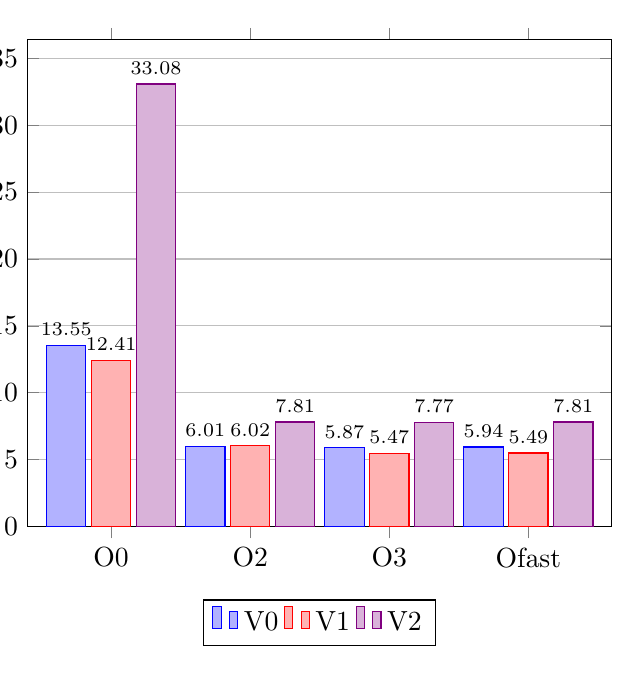
\begin{tikzpicture}[trim axis left, trim axis right]
    \begin{axis}[
            symbolic x coords={O0, O2, O3, Ofast},
            xtick = {O0, O2, O3, Ofast},
            legend style={at={(0.5,-0.15)},
                    anchor=north,legend columns=-1},
            ybar,
            ymin=0,
            ymajorgrids=true,
            ylabel=Seconds per iteration,
            bar width=5mm,
            width=90mm,
            enlarge x limits=0.2,
            nodes near coords,
            every node near coord/.append style={font = {\fontsize{7 pt}{12 pt}\selectfont},color=black},
        ]
        \addplot[blue,fill=blue!30]
        coordinates {(O0,13.55) (O2,6.01)
                (O3,5.87) (Ofast,5.94) };

        \addplot[red,fill=red!30]
        coordinates {(O0,12.41) (O2,6.02)
                (O3,5.47) (Ofast,5.49) };

        \addplot [violet,fill=violet!30]
        coordinates {(O0,33.08) (O2,7.81)
                (O3,7.77) (Ofast,7.81) };
        \legend{V0,V1,V2}
    \end{axis}
\end{tikzpicture}
\end{center}

Es wurden pro GCC-Optimierungsstufe und Implementierungsversion 5 
Iterationen des Verfahrens auf einer 1GB großen Datei ausgeführt.
Die Laufzeiten wurden vom Rahmenprogramm selbst durch setzen des -B Flags
gemessen. Getestet wurde auf einem Notebook mit einem AMD Ryzen 7 5800H, 
4.4GHz, 16 GiB Arbeitsspeicher, Fedora 36, 64 Bit, Linux Kernel 5.18.11.
Kompiliert wurde mit GCC 12.1.1.

\section{Zusammenfassung und Ausblick}

% TODO: Fuegen Sie Ihre Quellen der Datei Ausarbeitung.bib hinzu
% Referenzieren Sie diese dann mit \cite{}.
% Beispiel: CR2 ist ein Register der x86-Architektur~\cite{intel2017man}.
\bibliographystyle{plain}
\bibliography{Ausarbeitung}{}

\end{document}